\chapter[AWS Deployment]{AWS Deployment \\
\small{\textit{-- JGa, JGr, CS}}
\index{AWSDeployment} 
\index{Chapter!AWS Deployment}
\label{Chapter::AWSDeployment}}

\section{Steps taken to deploy website}

The link to the website can be found here: \url{https://mgn8mc4khh.us-east-2.awsapprunner.com/}
\\
After both installing AWS and creating accounts, here are the steps we took to deploy our website using AWS:

\begin{enumerate}

    \item Configured environment variables:
    \begin{lstlisting}[language=bash]
    export AWS_ACCOUNT_ID=<My Account ID>
    export AWS_REGION=us-east-2
    export ECR_REPO=myapp
    export IMAGE_TAG=v1
    export APP_NAME=my-apprunner-app
    export CONTAINER_PORT=3000
    \end{lstlisting}

    \item Authenticated Docker with Amazon ECR:
    \begin{lstlisting}[language=bash]
    aws ecr get-login-password --region $AWS_REGION --profile default \
    | docker login --username AWS --password-stdin $AWS_ACCOUNT_ID.dkr.ecr.$AWS_REGION.amazonaws.com
    \end{lstlisting}

    \item Created an ECR repository:
    \begin{lstlisting}[language=bash]
    aws ecr create-repository \
      --repository-name $ECR_REPO \
      --region $AWS_REGION \
      --profile default
    \end{lstlisting}

    \item Built our Docker image locally:
    \begin{lstlisting}[language=bash]
    docker build -t $ECR_REPO:$IMAGE_TAG .
    \end{lstlisting}

    \item Tagged the image for our private ECR repository:
    \begin{lstlisting}[language=bash]
    docker tag $ECR_REPO:$IMAGE_TAG \
    $AWS_ACCOUNT_ID.dkr.ecr.$AWS_REGION.amazonaws.com/$ECR_REPO:$IMAGE_TAG
    \end{lstlisting}

    \item Pushed the image to ECR:
    \begin{lstlisting}[language=bash]
    docker push $AWS_ACCOUNT_ID.dkr.ecr.$AWS_REGION.amazonaws.com/$ECR_REPO:$IMAGE_TAG
    \end{lstlisting}

    \item Deployed the image to App Runner:
    \begin{lstlisting}[language=bash]
    aws apprunner create-service \
      --service-name "$APP_NAME" \
      --region "$AWS_REGION" --profile default \
      --source-configuration "{
        \"ImageRepository\": {
          \"ImageIdentifier\": \"$AWS_ACCOUNT_ID.dkr.ecr.$AWS_REGION.amazonaws.com/$ECR_REPO:$IMAGE_TAG\",
          \"ImageRepositoryType\": \"ECR\",
          \"ImageConfiguration\": {\"Port\": \"$CONTAINER_PORT\"}
        },
        \"AuthenticationConfiguration\": {
          \"AccessRoleArn\": \"arn:aws:iam::$AWS_ACCOUNT_ID:role/AppRunnerECRAccessRole\"
        },
        \"AutoDeploymentsEnabled\": true
      }" \
      --instance-configuration "{\"Cpu\":\"1 vCPU\",\"Memory\":\"2 GB\"}"
    \end{lstlisting}

    \item Viewed the service status until it said \texttt{RUNNING}:
    \begin{lstlisting}[language=bash]
    aws apprunner describe-service \
      --service-arn arn:aws:apprunner:us-east-2:039612868337:service/my-apprunner-app/645d0eab8242460da212316afafce4ec \
      --region $AWS_REGION --profile default \
      --query 'Service.Status'
    \end{lstlisting}

    \item Once the status was \texttt{RUNNING}, we were able to access our live website using the \texttt{ServiceUrl} provided, e.g.:\\
    
    \url{https://mgn8mc4khh.us-east-2.awsapprunner.com}
\end{enumerate}



\section{Class Based Website}

\lstset{
  language=HTML,
  basicstyle=\ttfamily\footnotesize,
  keywordstyle=\color{blue},
  stringstyle=\color{red},
  commentstyle=\color{green!50!black},
  breaklines=true,
  showstringspaces=false,
  tabsize=2
}

\begin{lstlisting}[language=HTML]
<!DOCTYPE html>
<html lang="en">
<head>
  <meta charset="UTF-8">
  <title>Color Buttons App</title>
  <style>
    body {
      font-family: Arial, sans-serif;
      text-align: center;
      margin-top: 50px;
      transition: background-color 0.3s ease;
    }
    button {
      padding: 12px 24px;
      font-size: 18px;
      margin: 10px;
      cursor: pointer;
    }
  </style>
</head>
<body>
  <h1>Click a Button to Change Background</h1>
  <button id="blueBtn">Blue</button>
  <button id="redBtn">Red</button>

  <script>
    // Define a class to handle color changes
    class ColorChanger {
      constructor() {
        this.body = document.body;
        this.blueBtn = document.getElementById("blueBtn");
        this.redBtn = document.getElementById("redBtn");
      }

      init() {
        this.blueBtn.addEventListener("click", () => this.changeColor("blue"));
        this.redBtn.addEventListener("click", () => this.changeColor("red"));
      }

      changeColor(color) {
        this.body.style.backgroundColor = color;
      }
    }

    // Create and initialize the object
    const colorChanger = new ColorChanger();
    colorChanger.init();
  </script>
</body>
</html>
\end{lstlisting}


\begin{figure}[h]
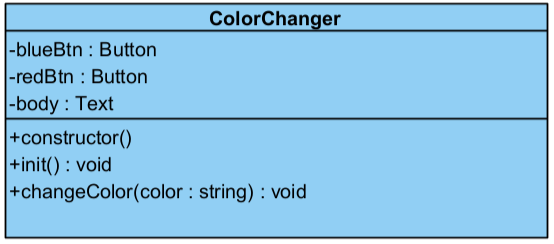
\includegraphics{png/ColorChangerUML.png}
\caption{UML diagram of class based Color Changer}
\centering
\end{figure}